\documentclass[tikz,border=1mm]{standalone}

\usepackage{amsmath}
\usepackage{graphicx}
\renewcommand\familydefault{\sfdefault} 
\usepackage[T1]{fontenc}

\usetikzlibrary{arrows,shapes,calc,math,decorations.fractals,patterns,backgrounds,decorations.markings}
\tikzset{every picture/.style={/utils/exec={\sffamily}}}
\tikzset{point/.style={fill,circle,inner sep=1.5pt}}
\tikzset{vel/.style={-triangle 45,blue!50!black,line width=1pt}}
\tikzset{acc/.style={-triangle 45,red,line width=1pt}}
\tikzset{myarrow/.style={decoration={markings,mark=at position 1 with %
    {\arrow[scale=3,>=stealth]{>}}},postaction={decorate}}}

\begin{document}

% 3D cartesian co-ordinates
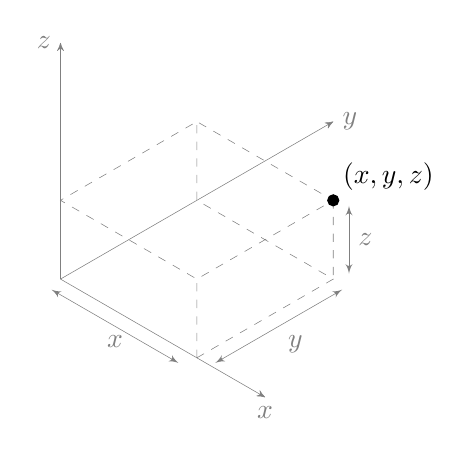
\begin{tikzpicture}
    \draw [-stealth',help lines] (0,0) -- (330:3) node [below] {$x$};
    \draw [-stealth',help lines] (0,0) -- (30:4) node [right] {$y$};
    \draw [-stealth',help lines] (0,0) -- (90:3) node [left] {$z$};
    \draw [help lines,dashed] (330:2) -- ++(30:2) -- ++(150:2) -- ++(90:1) -- ++(210:2) -- ++(330:2) -- ++(30:2) coordinate (p) -- ++(150:2) (p) -- ++(270:1) (330:2) -- ++(90:1);
    \draw [fill] (p) circle (2pt) node [above right] {$(x,y,z)$};
    \draw [latex'-latex',help lines,shorten <= 2pt,shorten >= 2pt] (210:0.2) -- node [below] {$x$} ++(330:2);
    \draw [latex'-latex',help lines,shorten <= 2pt,shorten >= 2pt] (330:2.2) -- node [below right] {$y$} ++(30:2);
    \draw [latex'-latex',help lines,shorten <= 2pt,shorten >= 2pt] ($(p)+(0:0.2)$) -- node [right] {$z$} ++(270:1);
\end{tikzpicture}

\end{document}